\documentclass[ignorenonframetext,]{beamer}
\setbeamertemplate{caption}[numbered]
\setbeamertemplate{caption label separator}{:}
\setbeamercolor{caption name}{fg=normal text.fg}
\usepackage{amssymb,amsmath}
\usepackage{ifxetex,ifluatex}
\usepackage{fixltx2e} % provides \textsubscript
\usepackage{lmodern}
\ifxetex
  \usepackage{fontspec,xltxtra,xunicode}
  \defaultfontfeatures{Mapping=tex-text,Scale=MatchLowercase}
  \newcommand{\euro}{€}
\else
  \ifluatex
    \usepackage{fontspec}
    \defaultfontfeatures{Mapping=tex-text,Scale=MatchLowercase}
    \newcommand{\euro}{€}
  \else
    \usepackage[T1]{fontenc}
    \usepackage[utf8]{inputenc}
      \fi
\fi
% use upquote if available, for straight quotes in verbatim environments
\IfFileExists{upquote.sty}{\usepackage{upquote}}{}
% use microtype if available
\IfFileExists{microtype.sty}{\usepackage{microtype}}{}
\usepackage{graphicx}
\makeatletter
\def\maxwidth{\ifdim\Gin@nat@width>\linewidth\linewidth\else\Gin@nat@width\fi}
\def\maxheight{\ifdim\Gin@nat@height>\textheight0.8\textheight\else\Gin@nat@height\fi}
\makeatother
% Scale images if necessary, so that they will not overflow the page
% margins by default, and it is still possible to overwrite the defaults
% using explicit options in \includegraphics[width, height, ...]{}
\setkeys{Gin}{width=\maxwidth,height=\maxheight,keepaspectratio}

% Comment these out if you don't want a slide with just the
% part/section/subsection/subsubsection title:
\AtBeginPart{
  \let\insertpartnumber\relax
  \let\partname\relax
  \frame{\partpage}
}
\AtBeginSection{
  \let\insertsectionnumber\relax
  \let\sectionname\relax
  \frame{\sectionpage}
}
\AtBeginSubsection{
  \let\insertsubsectionnumber\relax
  \let\subsectionname\relax
  \frame{\subsectionpage}
}

\setlength{\parindent}{0pt}
\setlength{\parskip}{6pt plus 2pt minus 1pt}
\setlength{\emergencystretch}{3em}  % prevent overfull lines
\setcounter{secnumdepth}{0}
\usetheme{Singapore} 
\usepackage{graphicx}
\usepackage{verbatim}
\usepackage{bm}
\usepackage[loop]{animate}
%\usepackage[usenames,dvipsnames,svgnames,table]{xcolor}
%\usepackage[usenames,dvipsnames]{xcolor}
%\graphicspath{{assets/}}
\usepackage{xmpmulti}
\usefonttheme[onlymath]{serif}
\usefonttheme{structurebold}
\usepackage{hyperref}

\setbeamersize{text margin left=6mm, text margin right=6mm} 

\def\slantfrac#1#2{\hbox{$\,^#1\!/_#2$}}

%% show frame number
%\setbeamertemplate{footline}{\scriptsize{\vspace*{0.3cm}\hspace*{0.1cm}\insertframenumber}} 

\setbeamertemplate{navigation symbols}{}%remove navigation symbols
\setbeamerfont{frametitle}{size=\large,series=\bfseries}
\setbeamerfont{alerted text}{series=\bfseries}

\title{Remote Sensing data}
\date{}

\begin{document}
\frame{\titlepage}

\section{Today}\label{today}

\subsection{}\label{section}

\begin{frame}{Projects}

First draft due next week.

\begin{itemize}
\itemsep1pt\parskip0pt\parsep0pt
\item
  upload \texttt{.Rmd} and \texttt{.pdf} (not HTML!)
\end{itemize}

Other questions?

\end{frame}

\begin{frame}{Objectives}

\begin{itemize}
\itemsep1pt\parskip0pt\parsep0pt
\item
  Brief introduction to remote sensing
\item
  Obtaining NASA remote sensing data
\item
  MODIS
\item
  MODIStools package
\end{itemize}

\end{frame}

\section{Remote sensing Introduction}\label{remote-sensing-introduction}

\subsection{}\label{section-1}

\begin{frame}{Active Earth Observing Satellites (EOS) (as of 8/31/2015)}

\begin{itemize}
\itemsep1pt\parskip0pt\parsep0pt
\item
  Total number of operating satellites: 1,305
\item
  Total Earth Observing Satellites (EOS): 333

  \begin{itemize}
  \itemsep1pt\parskip0pt\parsep0pt
  \item
    United States: 34\%
  \item
    China: 21\%\\
  \item
    Japan 6.3\%
  \end{itemize}
\end{itemize}

From the
\href{http://www.ucsusa.org/nuclear-weapons/space-weapons/satellite-database.html\#.VjzlnoS98VQ}{Union
of Concerned Scientists Satellite Database} and
\href{http://www.pixalytics.com/blog/}{Pixalytics Blog}

\end{frame}

\begin{frame}{Debris \& Satellites in low Earth orbit}

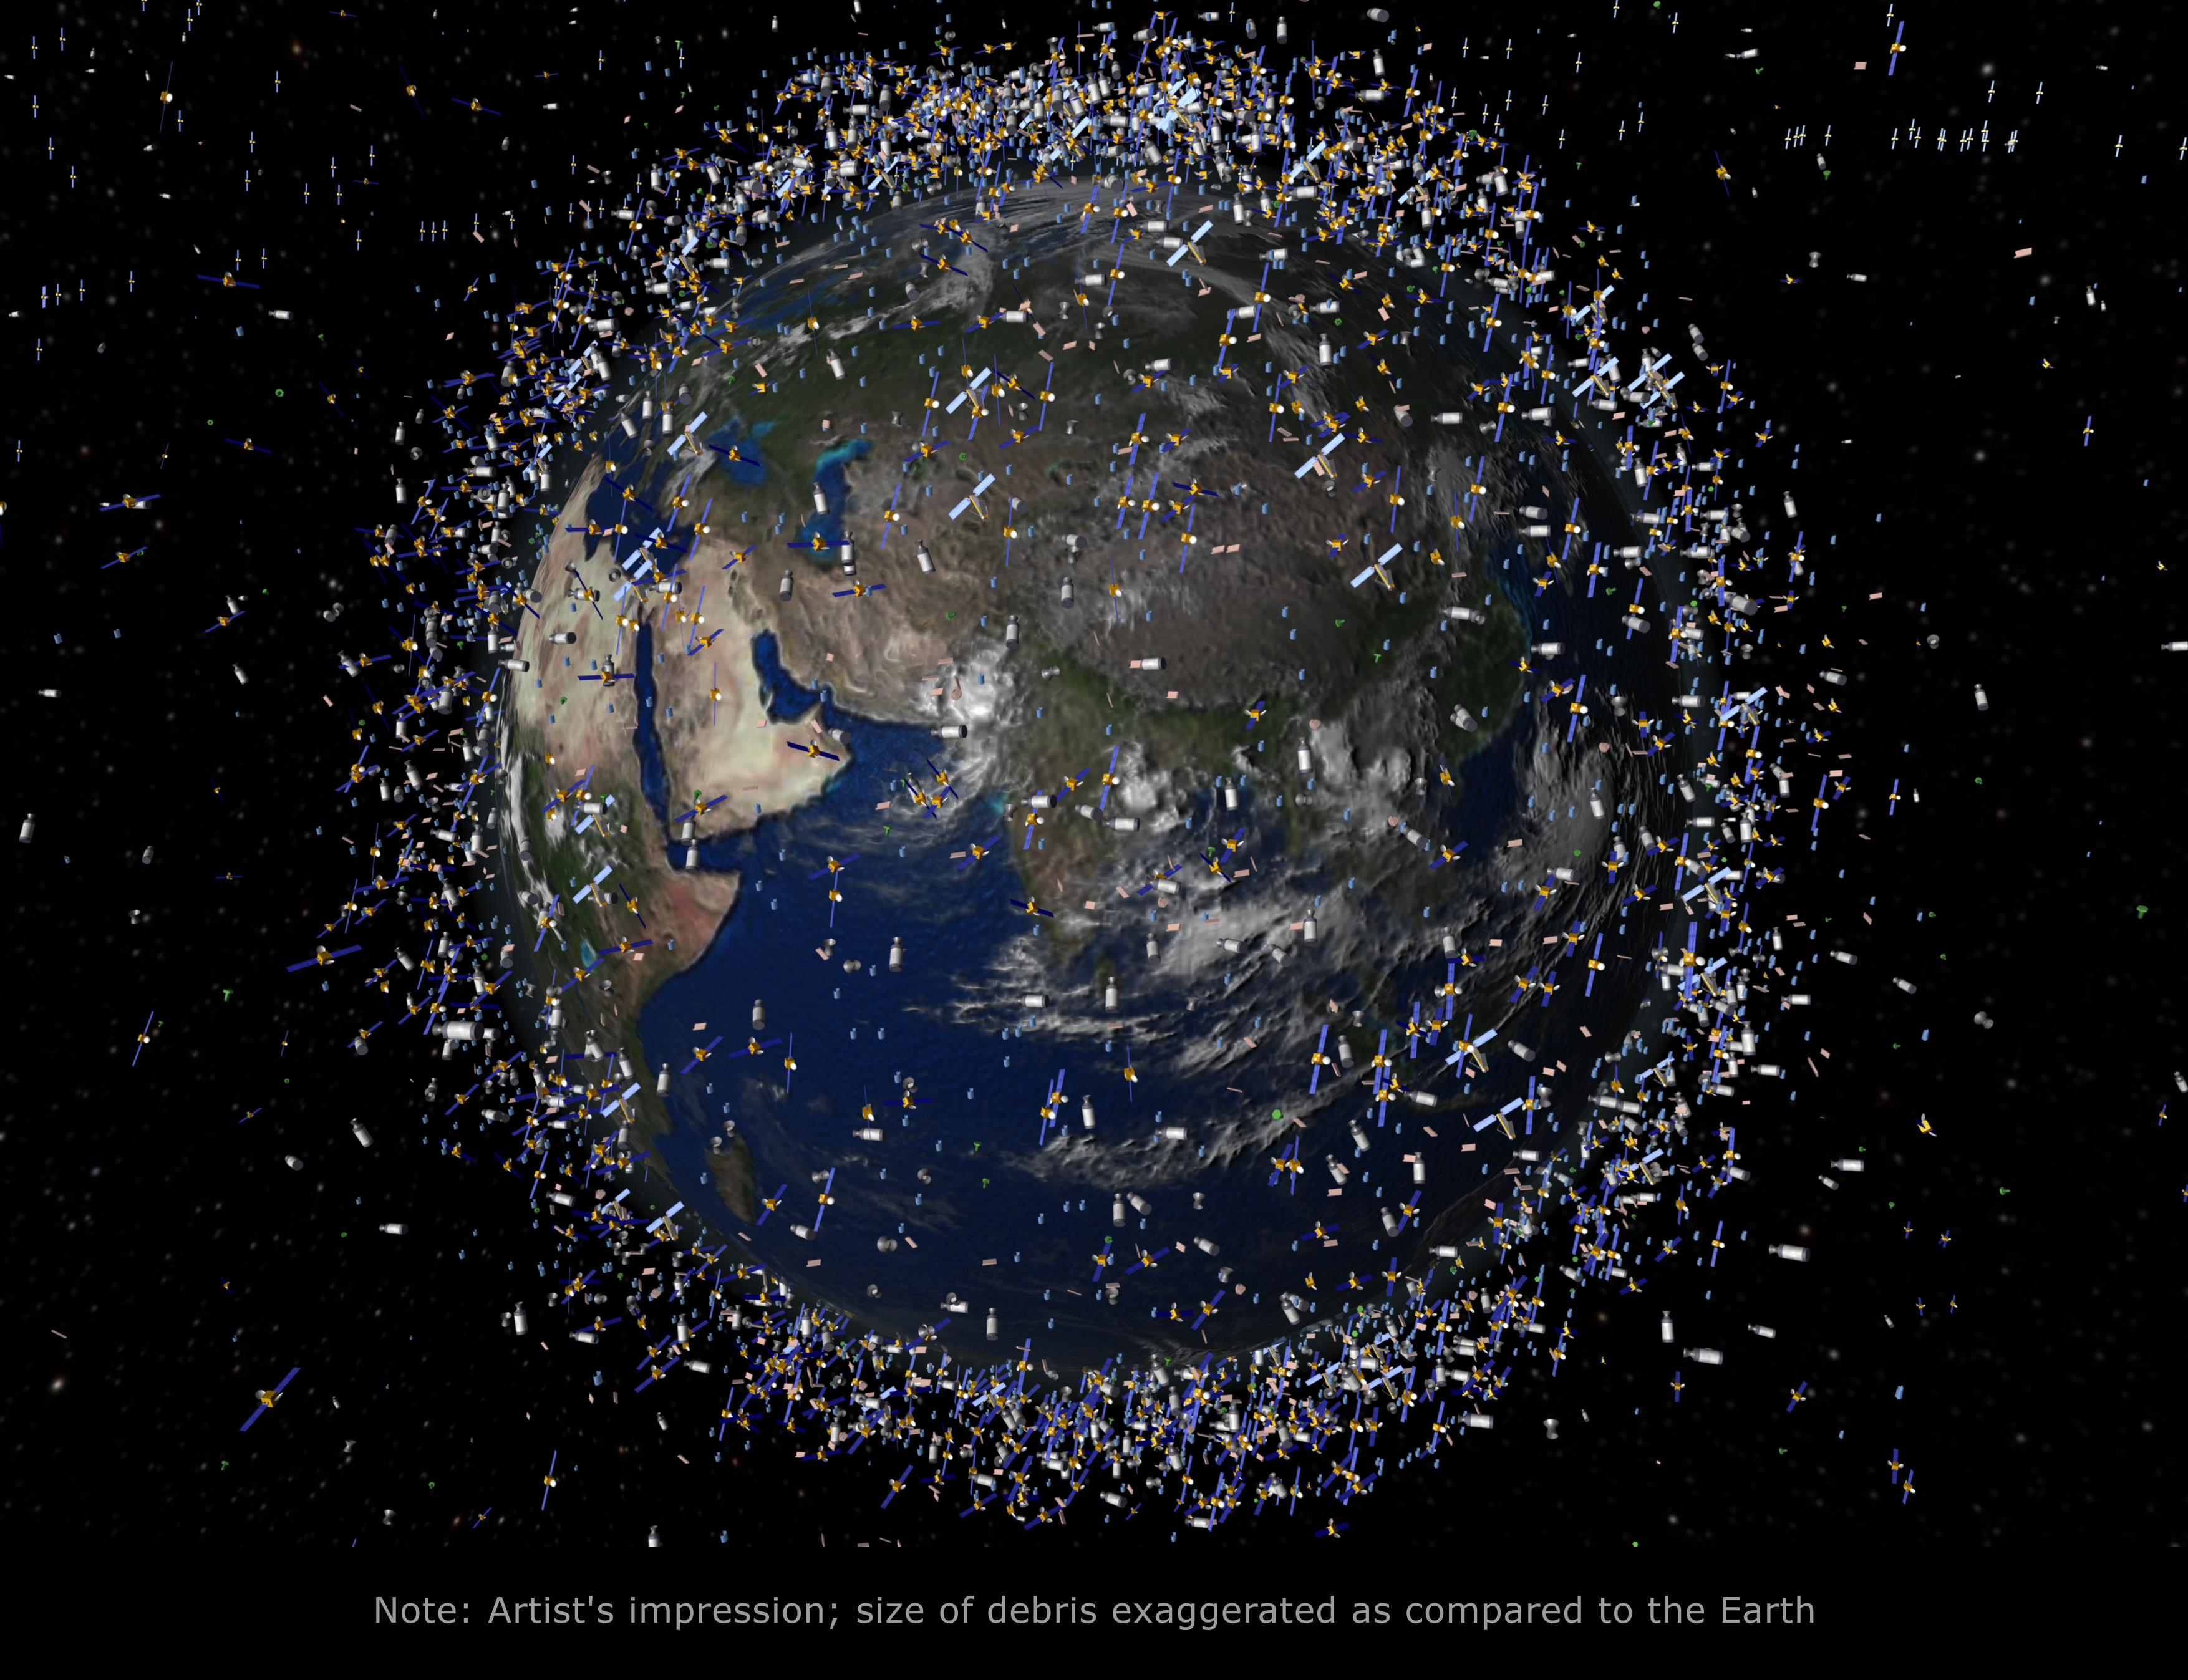
\includegraphics{assets/satellites.jpg}

Image courtesy of
\href{http://www.esa.int/spaceinimages/Images/2008/03/Debris_objects_-_mostly_debris_-_in_low_Earth_orbit_LEO_-_view_over_the_equator}{European
Space Agency}

\end{frame}

\begin{frame}{NASA's Earth Observing System}

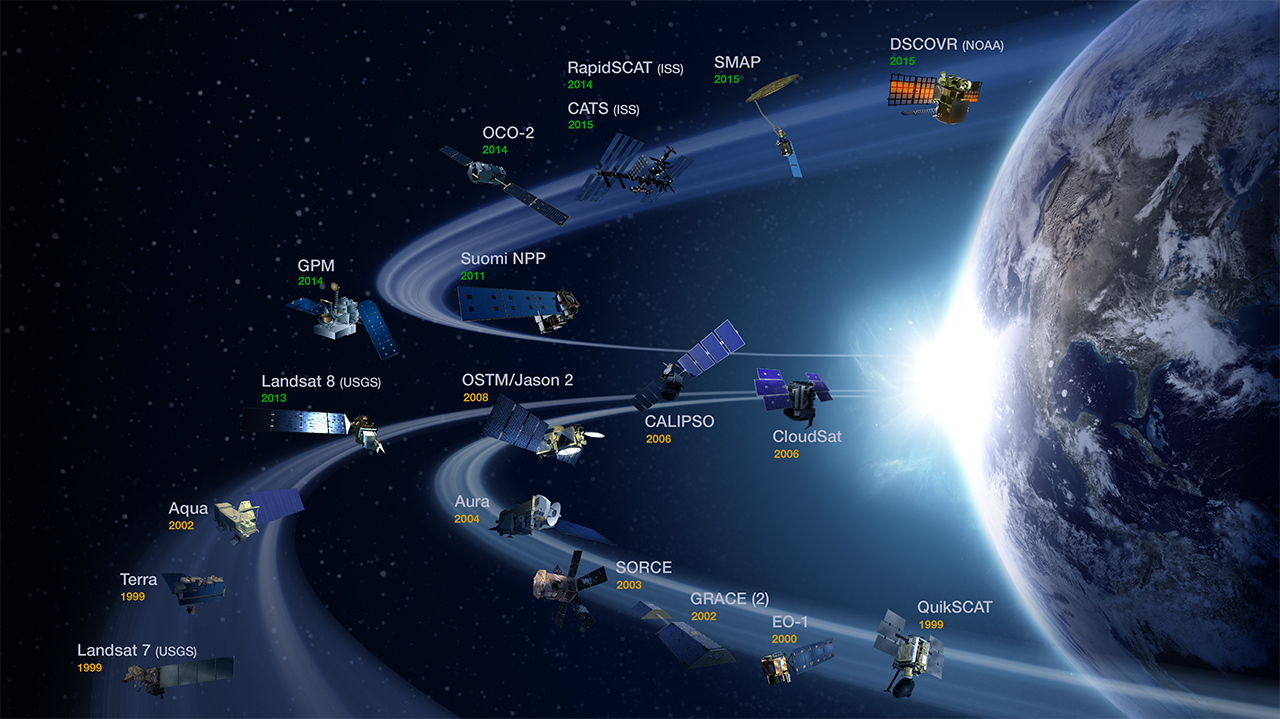
\includegraphics{assets/eos.jpg}

\end{frame}

\begin{frame}{Passive Remote Sensing}

\begin{block}{Electromagnetic Radiation}

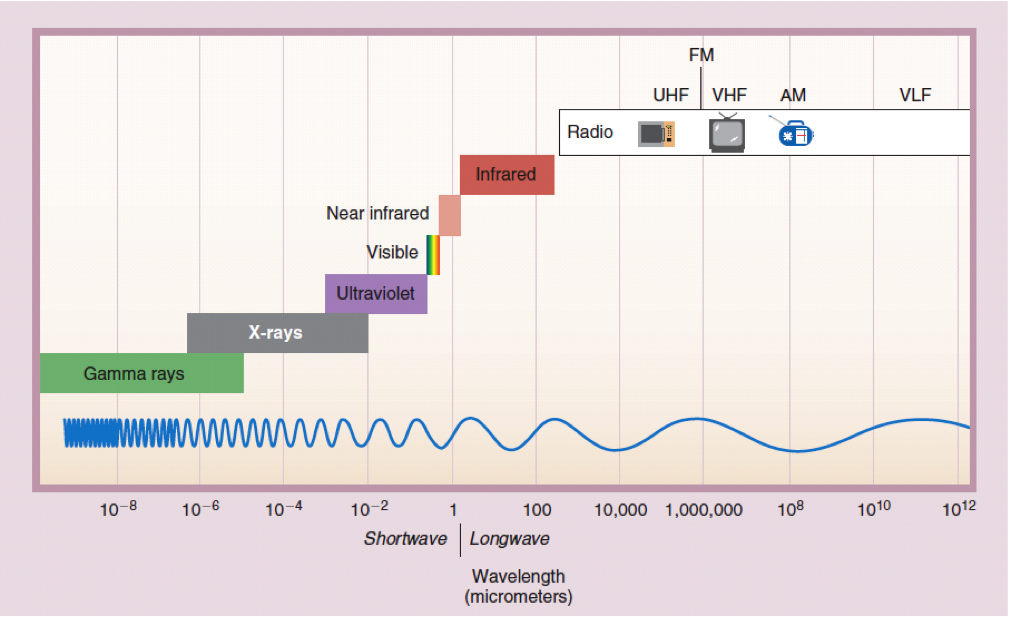
\includegraphics{assets/spectrum.png}

\end{block}

\end{frame}

\begin{frame}{\href{https://earthdata.nasa.gov}{EarthData.nasa.gov}}

Datasets, news, articles, information

\includegraphics{assets/Earthdata1.png}

\end{frame}

\begin{frame}{\href{https://earthdata.nasa.gov}{EarthData.nasa.gov}}

Datasets, news, articles, information

\includegraphics{assets/Earthdata2.png}

\end{frame}

\section{MODIS}\label{modis}

\subsection{}\label{section-2}

\begin{frame}{Moderate Resolution Imaging Spectroradiometer (MODIS)}

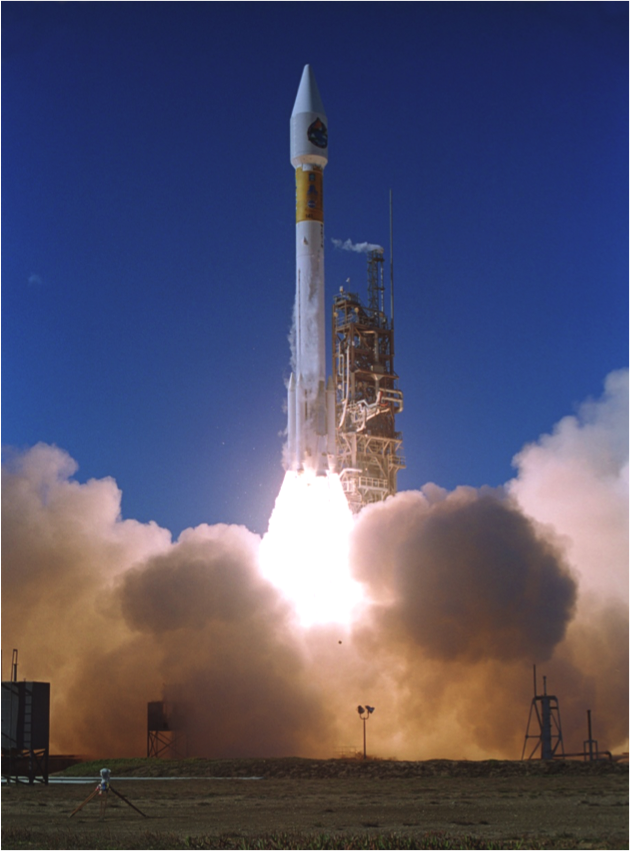
\includegraphics{assets/TerraLaunch.png}

2 Satellites \emph{Terra} launched in 1999, \emph{Aqua} in 2002.

\end{frame}

\begin{frame}{Technical Details: swath}

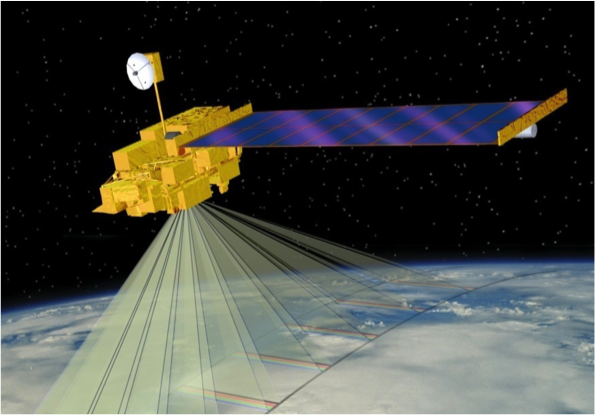
\includegraphics{assets/terra.png}

Viewing swath width of 2,330 km

\end{frame}

\begin{frame}{Technical Details: spatial coverage}

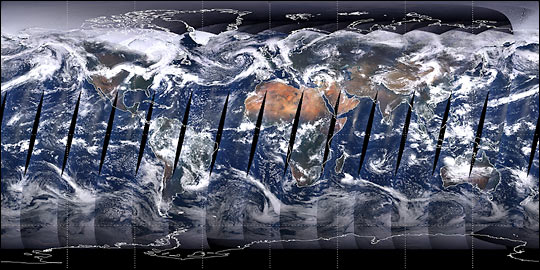
\includegraphics{assets/first_complete_day_from_modis.jpg}

Covers Earth every one to two days

\end{frame}

\begin{frame}{Technical Details: spectral coverage}

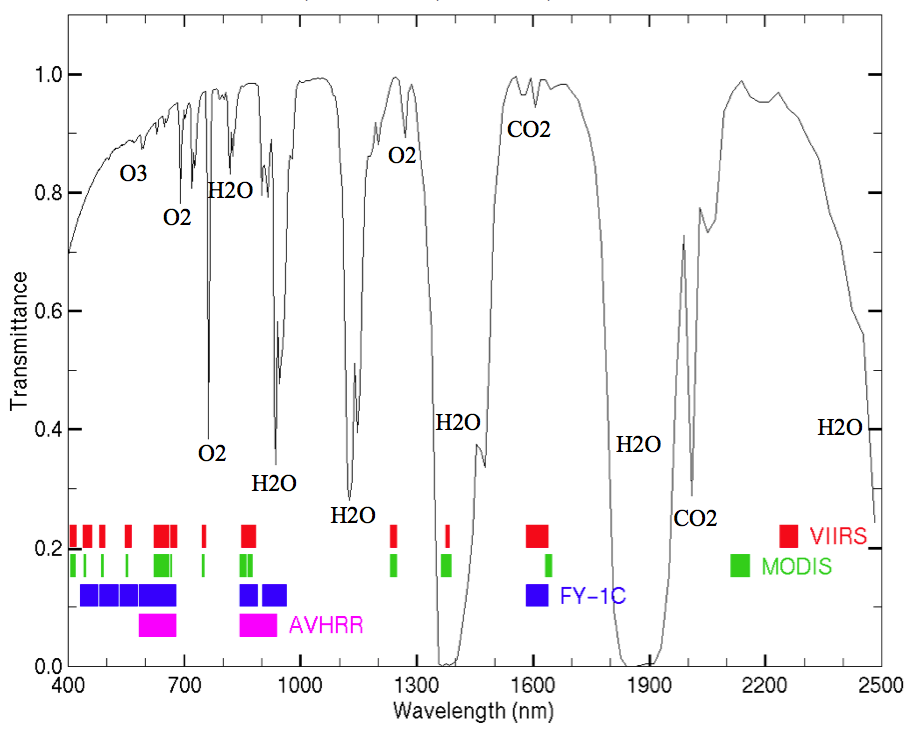
\includegraphics{assets/spectrum2.png}

36 spectral bands between 0.405 and 14.385 µm

\end{frame}

\begin{frame}{Technical Details: spatial resolution}

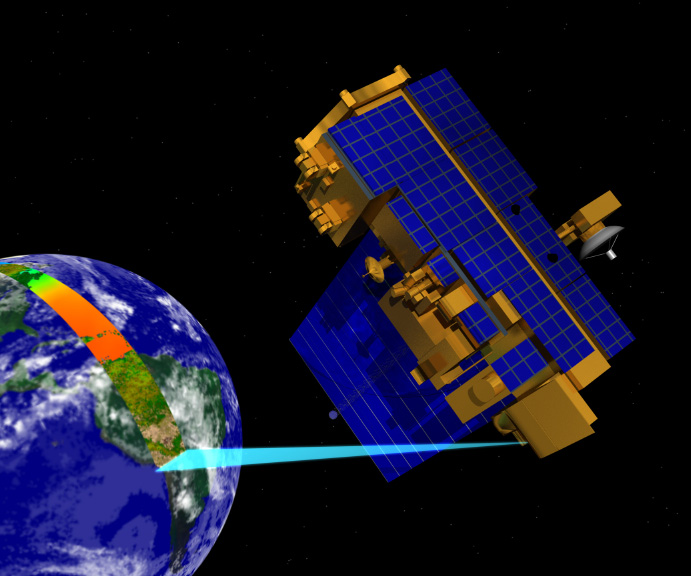
\includegraphics{assets/resolution.jpg}

3 spatial resolutions -- 250m, 500m, and 1,000m

\end{frame}

\begin{frame}{MODIS Data Processing}

\begin{itemize}
\itemsep1pt\parskip0pt\parsep0pt
\item
  Tracking and Data Relay Satellite System in White Sands, New Mexico
\item
  EOS Data and Operations System @ Goddard Space Flight Center in
  Greenbelt, MD
\item
  MODIS Adaptive Processing System (MODAPS)
\item
  3 DAACs for distribution
\end{itemize}

\end{frame}

\begin{frame}{MODIS products (a subset\ldots{})}

\begin{block}{Atmosphere}

\begin{itemize}
\itemsep1pt\parskip0pt\parsep0pt
\item
  Aerosol \& Clouds
\item
  Total Precipitable Water
\end{itemize}

\end{block}

\begin{block}{Cryosphere Products}

\begin{itemize}
\itemsep1pt\parskip0pt\parsep0pt
\item
  Snow Cover
\item
  Sea Ice and Ice Surface Temperature
\end{itemize}

\end{block}

\begin{block}{Ocean Products}

\begin{itemize}
\itemsep1pt\parskip0pt\parsep0pt
\item
  Sea Surface Temperature
\item
  Sub-surface Chlorophyll-a Concentration
\item
  Particulate Carbon
\item
  Photosynthetically Available Radiation
\end{itemize}

\end{block}

\end{frame}

\begin{frame}{Land Products}

\begin{itemize}
\itemsep1pt\parskip0pt\parsep0pt
\item
  Surface Reflectance
\item
  Land Surface Temperature and Emissivity
\item
  Land Cover Products
\item
  Vegetation Index Products (NDVI and EVI)
\item
  Thermal Anomalies - Active Fires
\item
  Photosynthetically Active Radiation (FPAR) / Leaf Area Index (LAI)
\item
  Evapotranspiration
\item
  Primary Productivity
\item
  Vegetation Continuous Fields
\item
  Water Mask
\item
  Burned Area Product
\end{itemize}

\end{frame}

\begin{frame}{Example product workflow}

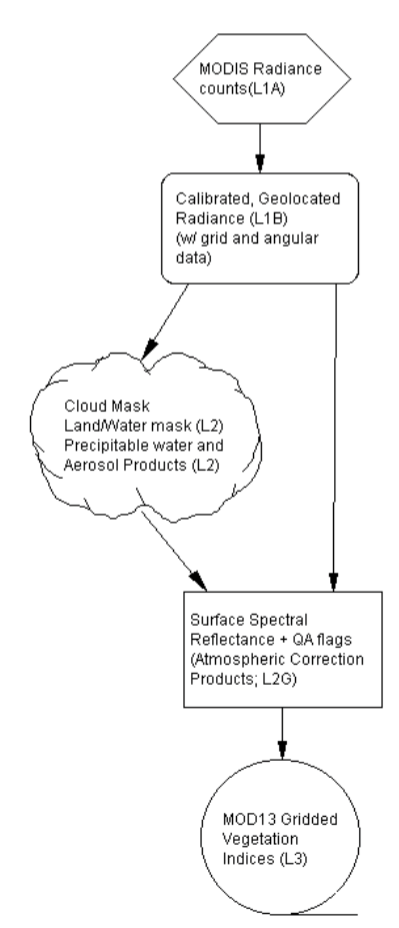
\includegraphics{assets/VI_flow.png}

MODIS Products used to generate vegetation indices. From the
\href{http://modis.gsfc.nasa.gov/data/atbd/atbd_mod13.pdf}{MOD13
Algorithm Theoretical Basis Document}.

\end{frame}

\begin{frame}{Data formats}

Most NASA EOS data distributed as HDF files, which are very similar to
netCDF.

\includegraphics{assets/NETCDF4Library.jpg}

\end{frame}

\begin{frame}{NetCDF / HDF}

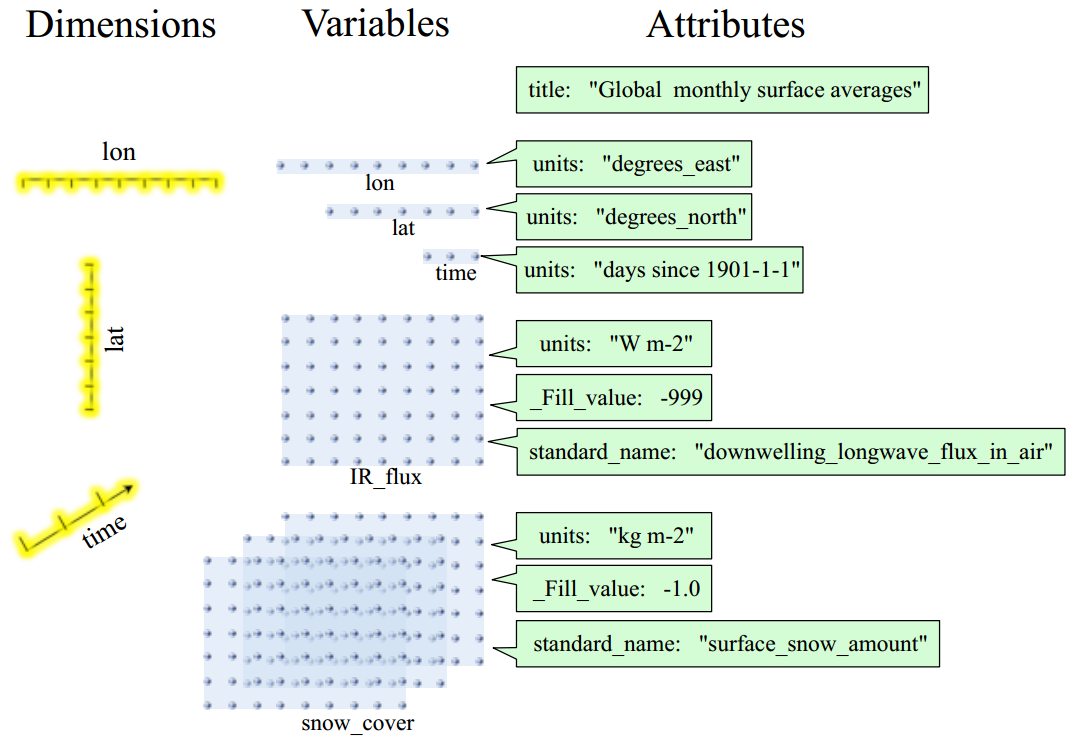
\includegraphics{assets/netcdf2.png}

\end{frame}

\begin{frame}{Collection-Level Naming Conventsions}

\texttt{MODIS/Terra Surface Reflectance 8-Day L3 Global 500m SIN Grid V005}

\begin{itemize}
\itemsep1pt\parskip0pt\parsep0pt
\item
  \texttt{MODIS/Terra} - Instrument/Sensor
\item
  \texttt{Surface Reflectance} - Geophysical Parameter
\item
  \texttt{8-Day} - Temporal Resolution
\item
  \texttt{L3} - Processing Level
\item
  \texttt{Global} - Global or Swath
\item
  \texttt{500m} - Spatial Resolution
\item
  \texttt{SIN Grid} - Gridded or Not
\item
  \texttt{V005} - Collection Version
\end{itemize}

\end{frame}

\begin{frame}{MODIS Gridding system}

\includegraphics{assets/modgrid.gif}

\end{frame}

\begin{frame}{Filename Conventions}

\texttt{MOD09A1.A2006001.h08v05.005.2006012234657.hdf}

\begin{itemize}
\itemsep1pt\parskip0pt\parsep0pt
\item
  \texttt{MOD09A1} - Product Short Name
\item
  \texttt{.A2006001} - Julian Date of Acquisition (A-YYYYDDD)
\item
  \texttt{.h08v05} - Tile Identifier (horizontalXXverticalYY)
\item
  \texttt{.005} - Collection Version
\item
  \texttt{.2006012234567} - Julian Date of Production (YYYYDDDHHMMSS)
\item
  \texttt{.hdf} - Data Format (HDF-EOS)
\end{itemize}

\end{frame}

\begin{frame}{MODIS Temporal Resolution}

\begin{itemize}
\itemsep1pt\parskip0pt\parsep0pt
\item
  Daily
\item
  8-Day
\item
  16-Day
\item
  Monthly
\item
  Quarterly
\item
  Yearly
\end{itemize}

\end{frame}

\begin{frame}{MODIS Spatial Resolution}

\begin{itemize}
\itemsep1pt\parskip0pt\parsep0pt
\item
  \textbf{Bands 1--2} 250-meter
\item
  \textbf{Bands 3--7} 500-meter
\item
  \textbf{Bands 8--36} 1000-meter
\end{itemize}

\end{frame}

\section{MODIS Data}\label{modis-data}

\subsection{}\label{section-3}

\begin{frame}{Distributed Active Archive Centers (DAACs)}

\begin{itemize}
\itemsep1pt\parskip0pt\parsep0pt
\item
  \textbf{Level 1 data:} geolocation, cloud mask, and atmosphere
  products
  \href{http://ladsweb.nascom.nasa.gov/}{ladsweb.nascom.nasa.gov}
\item
  \textbf{Land products:}
  \href{https://lpdaac.usgs.gov/}{lpdaac.usgs.gov}
\item
  \textbf{Cryosphere (snow/ice) products:}
  \href{http://nsidc.org/daac/modis/index.html}{nsidc.org/daac/modis}
\item
  \textbf{Ocean color and sea surface temperature:}
  \href{http://oceancolor.gsfc.nasa.gov/}{oceancolor.gsfc.nasa.gov}
\end{itemize}

\end{frame}

\begin{frame}{Accessing data}

The Land Processes Distributed Active Archive Center has a nice ``Data
Discovery'' Tool: 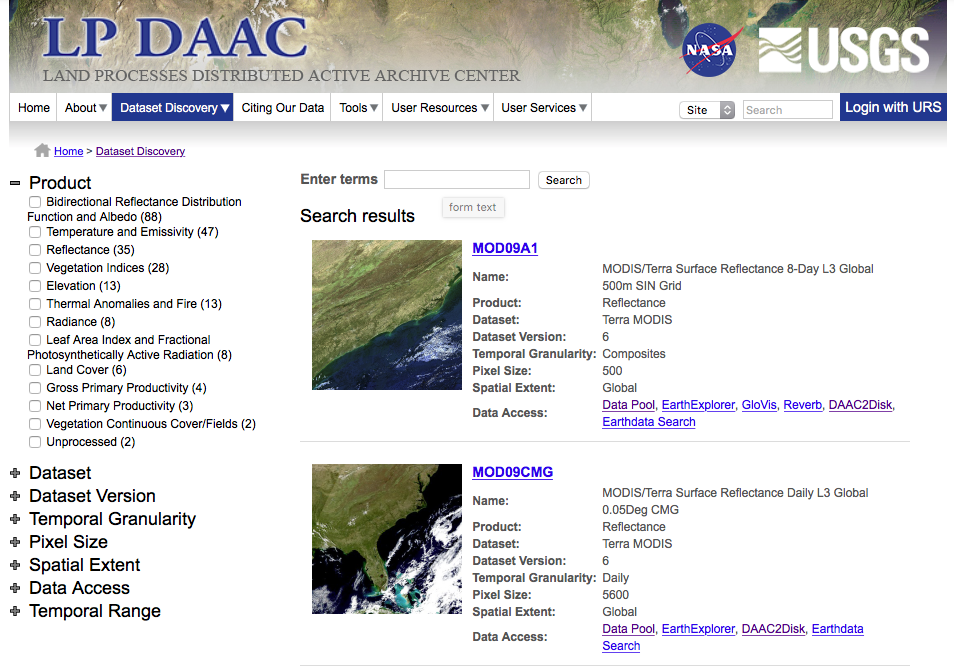
\includegraphics{assets/lpdaac.png}

\end{frame}

\begin{frame}{MODIS Products Table}

Lists \href{}{all available MODIS land products}

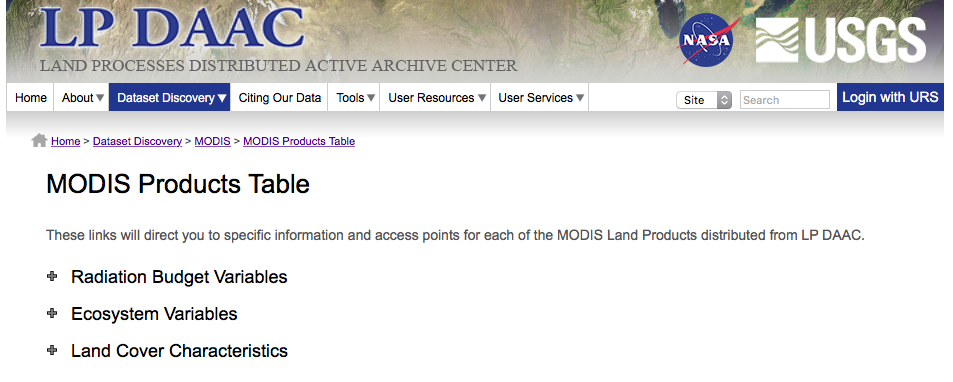
\includegraphics{assets/lpdaac1.png}

\end{frame}

\begin{frame}{Annual Land Cover Type Description}

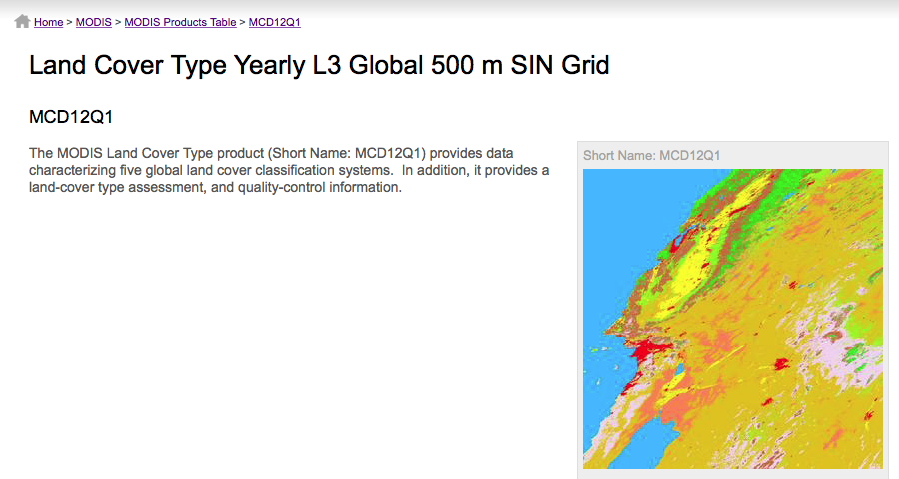
\includegraphics{assets/lpdaac2.png}

\end{frame}

\begin{frame}{Detailed layer information}

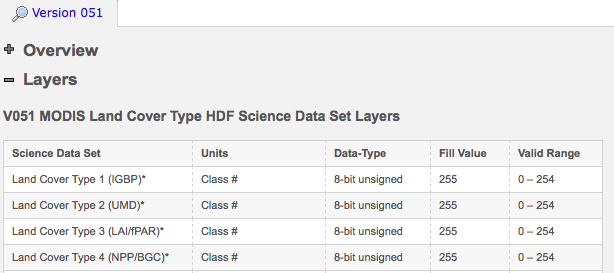
\includegraphics{assets/lpdaac3.png}

\end{frame}

\begin{frame}{Data access links}

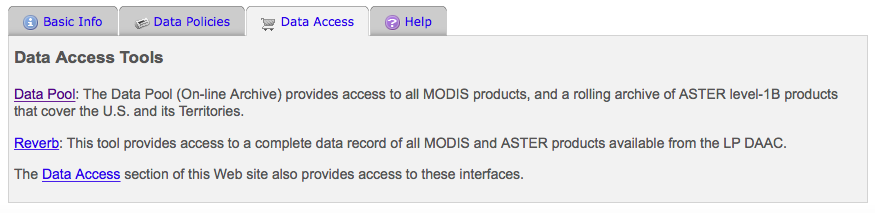
\includegraphics{assets/lpdaac4.png}

\end{frame}

\begin{frame}{Downloading: \texttt{http}/\texttt{ftp} access}

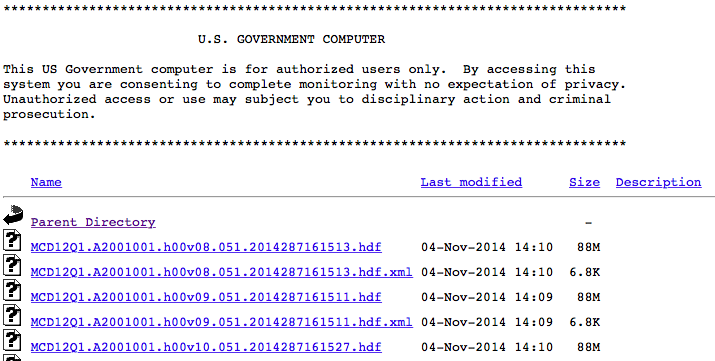
\includegraphics{assets/lpdaac5.png}

or the
\href{https://lpdaac.usgs.gov/sites/default/files/public/datapool/DAAC2DiskUserGuide.pdf}{LP
DAAC2Disk Download Manager} which builds a download script.

\end{frame}

\begin{frame}{MODIS Reprojection Tool}

Available at
\href{https://lpdaac.usgs.gov/tools/modis_reprojection_tool}{lpdaac.usgs.gov/tools/modis\_reprojection\_tool}.

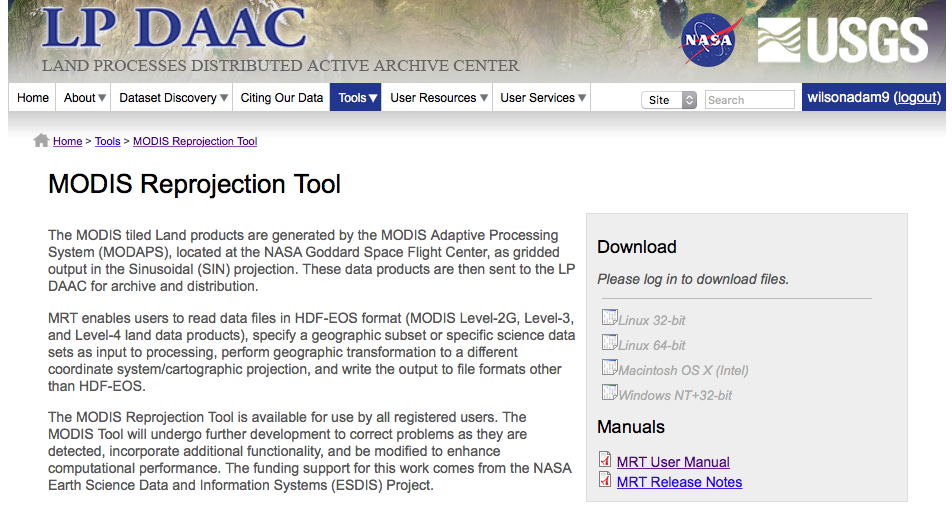
\includegraphics{assets/MRT1.png}

\end{frame}

\begin{frame}{MODIS Reprojection Tool: Subset \& Reproject}

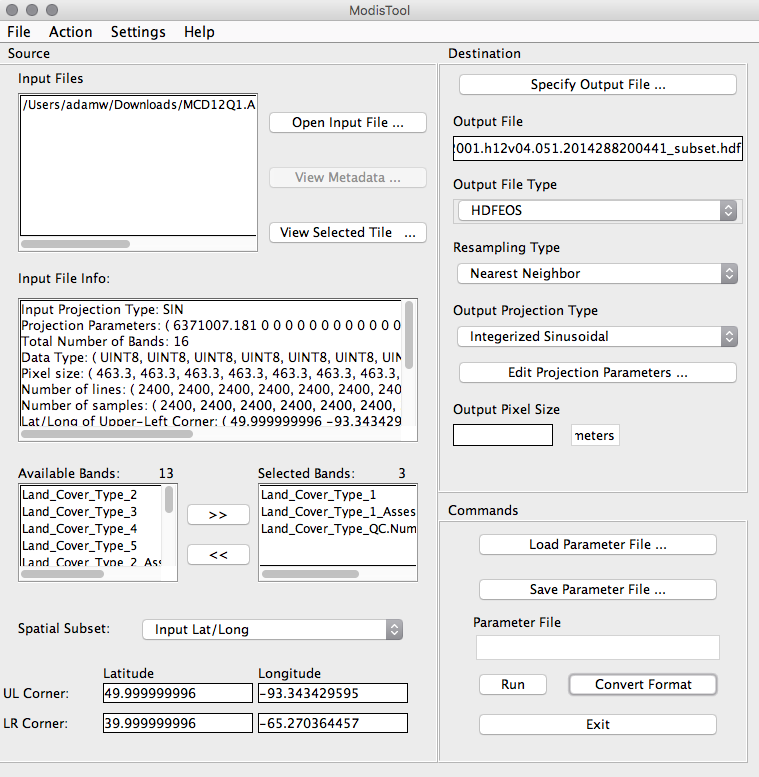
\includegraphics{assets/MRT.png}

\texttt{MCD12Q1.A2012001.h12v04.051.2014288200441.hdf}

\end{frame}

\begin{frame}{MODIS Web Services}


\includegraphics{assets/mws.png}

\href{http://daacmodis.ornl.gov/cgi-bin/MODIS/GLBVIZ_1_Glb/modis_subset_order_global_col5.pl}{daacmodis.ornl.gov/cgi-bin/MODIS/GLBVIZ\_1\_Glb/modis\_subset\_order\_global\_col5.pl}

\begin{itemize}
\itemsep1pt\parskip0pt\parsep0pt
\item
  Provide access to regional subsets (\textless{}100x100km)
\item
  Merge across tiles
\item
  Download full time series
\end{itemize}

\end{frame}

\begin{frame}{MODIS Subset: Spatial}

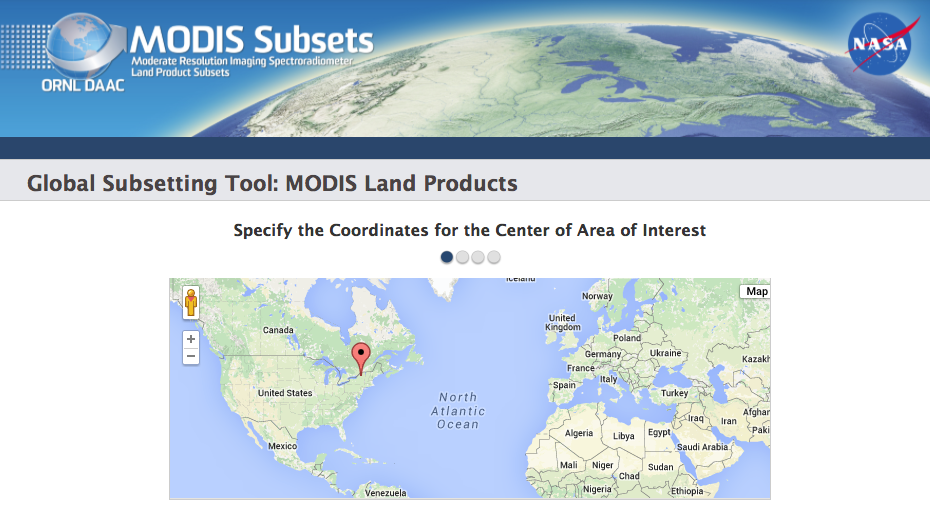
\includegraphics{assets/mws0.png}

\end{frame}

\begin{frame}{MODIS Subset: Variables}

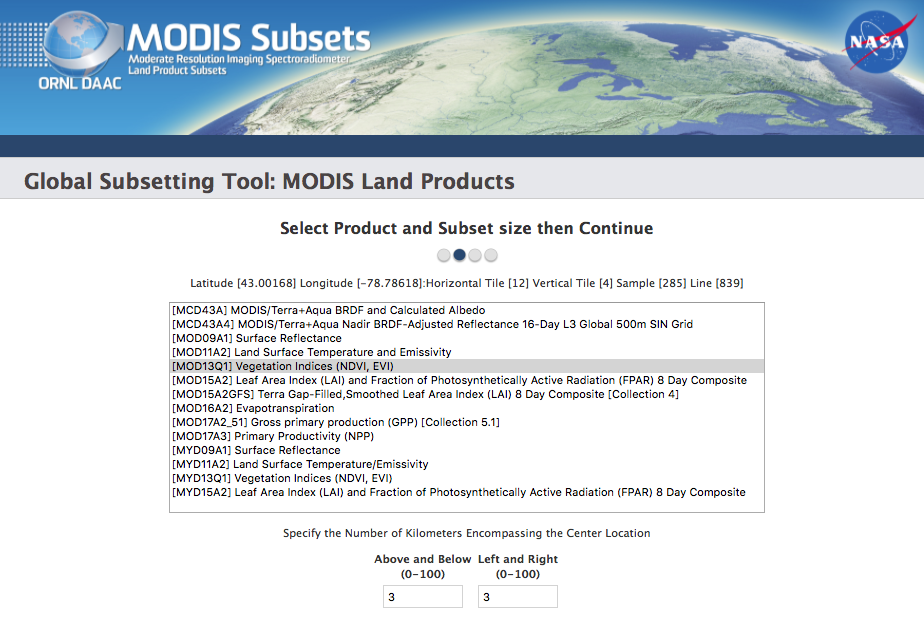
\includegraphics{assets/mws0b.png}

\end{frame}

\begin{frame}{MODIS Subset: Temporal}

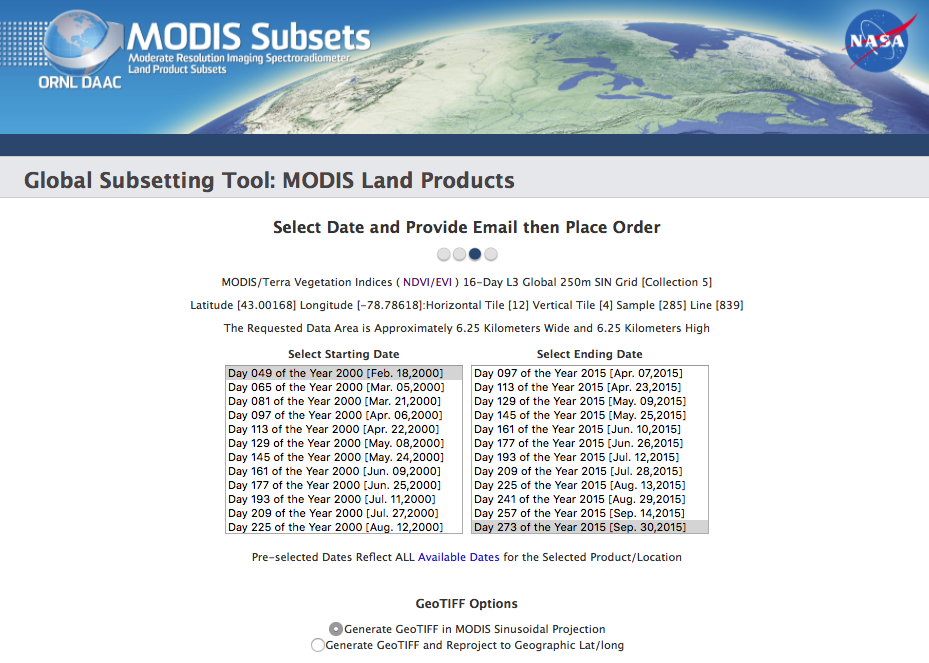
\includegraphics{assets/mws0c.png}

Submit email and wait for results\ldots{}

\end{frame}

\begin{frame}{MODIS Subset: Results \& Download}

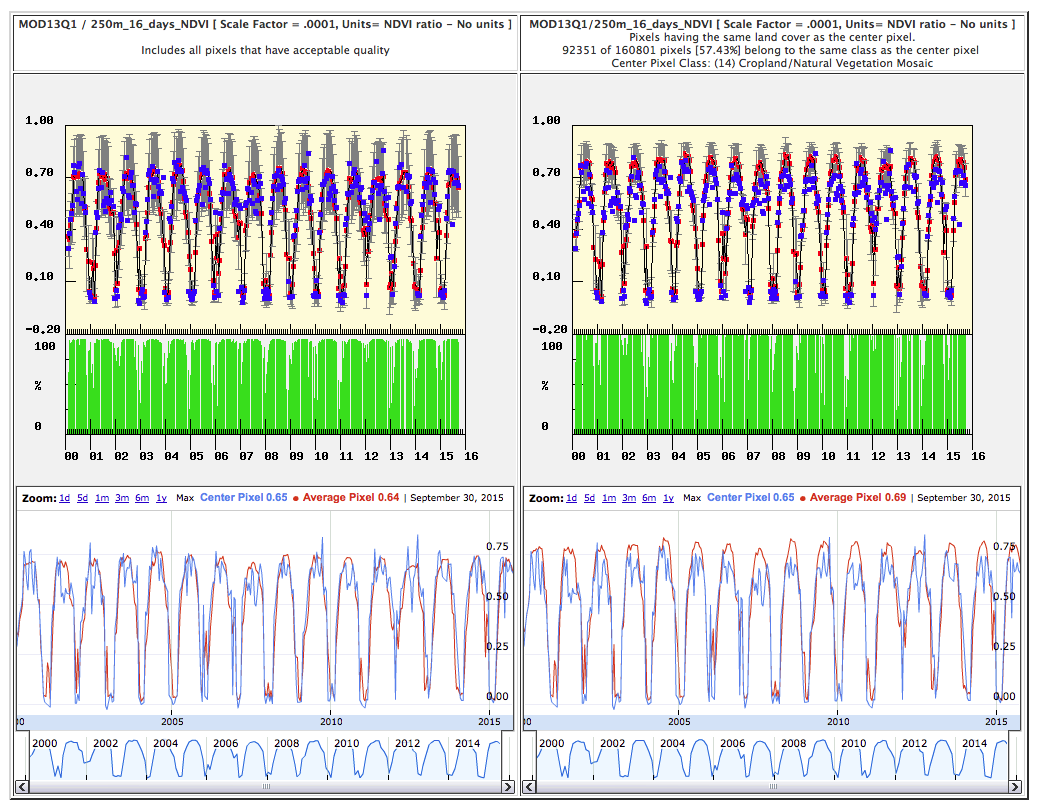
\includegraphics{assets/mws1.png}

\end{frame}

\begin{frame}{MODIS Subsets: API}

Subsets of MODIS Land Products through \textbf{Simple Object Access
Protocol} (\texttt{SOAP}).

\texttt{MODISTools} R package.

\end{frame}

\begin{frame}{Presentation Credits}

\begin{itemize}
\itemsep1pt\parskip0pt\parsep0pt
\item
  Images: NASA
\item
  Some contents from Steve Ackerman \texttt{stevea@ssec.wisc.edu},
  Cooperative Institute for Meteorological Satellite Studies, University
  of Wisconsin-Madison
\end{itemize}

\end{frame}

\end{document}
